\documentclass[11pt]{article}

\usepackage[margin=1in]{geometry}
\usepackage[T1]{fontenc}
\usepackage[utf8]{inputenc}
\usepackage{lmodern}
\usepackage{microtype}
\usepackage{amsmath, amssymb}
\usepackage{booktabs}
\usepackage{graphicx}
\usepackage{hyperref}
\usepackage{url}
\usepackage{enumitem}
\usepackage{xcolor}
\usepackage{listings}
\usepackage{tikz}
\usepackage{float}
\usepackage{tabularx}
\usepackage[numbers]{natbib}
\usetikzlibrary{positioning}

\hypersetup{
  colorlinks=true,
  linkcolor=blue,
  citecolor=blue,
  urlcolor=blue,
  pdftitle={SQLRite: Embedded-First SQL-Native Retrieval for Local-First AI Agents},
  pdfauthor={James Karanja Maina}
}

\lstdefinelanguage{SQLRiteSQL}{
  morekeywords={SELECT, FROM, WHERE, ORDER, BY, LIMIT, AS, WITH, CREATE, TABLE, INDEX, SEARCH, EXPLAIN, RETRIEVAL},
  sensitive=false,
  morecomment=[l]{--},
  morestring=[b]"
}

\lstset{
  basicstyle=\ttfamily\small,
  keywordstyle=\bfseries\color{blue!60!black},
  commentstyle=\itshape\color{gray!80!black},
  frame=single,
  breaklines=true,
  columns=fullflexible
}

\title{SQLRite: Embedded-First SQL-Native Retrieval for Local-First AI Agents}
\author{James Karanja Maina \\ Zavora Technologies Ltd \\ \texttt{james.karanja@zavora.ai}}
\date{March 2026}

\begin{document}
\maketitle

\begin{abstract}
AI-agent and retrieval-augmented generation systems often need retrieval that is embeddable, inspectable, SQL-accessible, and operationally simple. SQLRite is a Rust implementation of a SQLite-based retrieval engine that treats retrieval as part of the database surface rather than as a separate external service. The system combines lexical, vector, and hybrid retrieval with deterministic tie-breaking, a SQL-native retrieval layer, optional HTTP/gRPC/MCP interfaces, and operational capabilities such as ingest, reindex, backup, restore, migration, and security controls. This paper describes SQLRite's architecture and evaluates it in the deployment regime it is designed for: embedded local-first retrieval. On a deterministic filtered cosine workload with 5,000 records, 120 measured queries, 64 dimensions, and 8 tenants, SQLRite achieved 3380.07 queries/s in embedded exact mode and 3530.96 queries/s in embedded HNSW mode, both with Recall@10 = 1.0. On the same workload, compact HTTP preserved much of the gain, reaching 1807.27 and 1828.17 queries/s respectively. In that benchmark snapshot, SQLRite outperformed sqlite-vec exact (3163.27 queries/s), Qdrant exact (2576.75 queries/s), Qdrant HNSW (2661.91 queries/s), pgvector exact (1739.64 queries/s), pgvector HNSW (1924.01 queries/s, Recall@10 = 0.5740), and LanceDB IVF\_FLAT (1331.18 queries/s, Recall@10 = 0.9510). On a refreshed public benchmark over BEIR/SciFact using deterministic local embeddings, SQLRite exact compact HTTP reached 204.76 queries/s, while SQLRite hybrid compact HTTP reached 55.60 queries/s with Recall@10 = 0.4028 and NDCG@10 = 0.3973, exceeding a pgvector hybrid baseline at 23.66 queries/s, Recall@10 = 0.2278, and NDCG@10 = 0.1609 in the same harness. These results position SQLRite as an embedded-first retrieval engine that can compete credibly on performance while differentiating through SQL-native retrieval, deterministic execution, and a unified operational surface.
\end{abstract}

\section{Introduction}
Retrieval is becoming a default subsystem for AI agents, local memory layers, and retrieval-augmented generation pipelines \citep{lewis2020rag}. In many real deployments, however, retrieval still arrives as a collection of loosely coupled pieces: a storage engine, a text index, a vector index, an application-specific ranking layer, and one or more separate service boundaries. That separation is workable at scale, but it creates friction for teams that want something smaller, more inspectable, and easier to ship inside an application.

SQLRite is motivated by a narrower but increasingly important requirement: local-first retrieval for agent systems. The default deployment is not a cluster. It is a local database file, a library call, or a CLI command. When needed, the same engine can also be exposed through HTTP, gRPC, or Model Context Protocol (MCP), but the center of gravity remains embedded execution.

SQLite has already demonstrated the value of the single-file database model for a vast range of application workloads \citep{hipp2022sqlite}. SQLRite extends that philosophy toward retrieval. It preserves SQLite's inspectability and operational simplicity while adding retrieval-specific indexing, hybrid ranking, SQL-native retrieval operators, and application-facing transport surfaces.

This paper makes four contributions:
\begin{enumerate}[leftmargin=*, itemsep=0.2em]
  \item It presents SQLRite as an embedded-first retrieval architecture built on SQLite and implemented in Rust.
  \item It describes a SQL-native retrieval model that exposes vector operators, helper functions, and a \texttt{SEARCH(...)} abstraction directly in the query surface.
  \item It evaluates SQLRite in the regime it is designed for: deterministic, local-first, filtered retrieval with both embedded and low-overhead served access paths.
  \item It shows that SQLRite's strongest current story is not only operational simplicity, but also competitive embedded performance on a representative filtered workload and materially stronger hybrid retrieval quality on a public benchmark.
\end{enumerate}

\section{Problem Setting and Design Goals}
SQLRite is intended for developers building agent memory, local RAG, desktop knowledge tools, and edge-friendly retrieval services. These workloads differ from large distributed search deployments in three important ways.

First, they value \textbf{embedding} over centralization. The retrieval engine should live inside the application when possible, not force a separate service cluster by default. Second, they value \textbf{inspectability and determinism}. Developers need to understand why a chunk was returned, reproduce the behavior in tests, and inspect the state with familiar tools. Third, they often need \textbf{operational completeness} without operational sprawl: backup, restore, migration, reindex, security, and agent-facing APIs should exist in the same product boundary.

These goals lead to the following design requirements:
\begin{itemize}[leftmargin=*, itemsep=0.2em]
  \item \textbf{Embedded-first execution.} The best path should be in-process use against a local file or in-memory database.
  \item \textbf{SQL-native retrieval.} Developers should express retrieval in SQL, not only through out-of-band SDK calls.
  \item \textbf{Deterministic retrieval behavior.} Repeated runs on the same data should be stable enough for debugging and regression testing.
  \item \textbf{Transport flexibility.} The same engine should still support HTTP, compact HTTP, gRPC, and MCP when a process boundary is needed.
  \item \textbf{Operational cohesion.} Migration, backup, reindex, security, and maintenance should be first-class product surfaces.
\end{itemize}

The goal is not to replace every distributed vector database. The goal is to close the gap between ``an embedded SQLite database'' and ``a retrieval system suitable for AI agents.''

\section{Related Systems}
SQLRite sits between several well-known system categories. pgvector adds vector similarity search to PostgreSQL and is the most natural SQL-first comparison point \citep{pgvector2026}. Qdrant represents a network-native vector database optimized for filtered vector search and service deployment \citep{qdrant2026}. sqlite-vec extends SQLite toward embedded vector retrieval, making it the closest local-first comparator in spirit \citep{sqlitevec2026}. LanceDB spans local and server-backed usage and is relevant because it occupies an adjacent design space between embedded convenience and vector-oriented APIs \citep{lancedb2026}.

These systems solve related but not identical problems. Some optimize for distributed ANN throughput, some for database integration, and some for local application embedding. SQLRite's claim is narrower: it targets embedded-first retrieval while exposing richer SQL-native retrieval semantics and a broader in-product operational surface.

\section{System Overview}
At a high level, SQLRite combines five layers:
\begin{enumerate}[leftmargin=*, itemsep=0.2em]
  \item SQLite-backed persistence for chunks, metadata, document state, and FTS indexes,
  \item lexical and vector retrieval paths,
  \item a ranking layer supporting exact, ANN, weighted hybrid fusion, and reciprocal rank fusion,
  \item operational workflows such as ingest, reindex, migration, backup, and restore,
  \item multiple access surfaces: embedded library, CLI, HTTP, compact HTTP, gRPC, and MCP.
\end{enumerate}

\begin{figure}[H]
  \centering
  \resizebox{\linewidth}{!}{%
  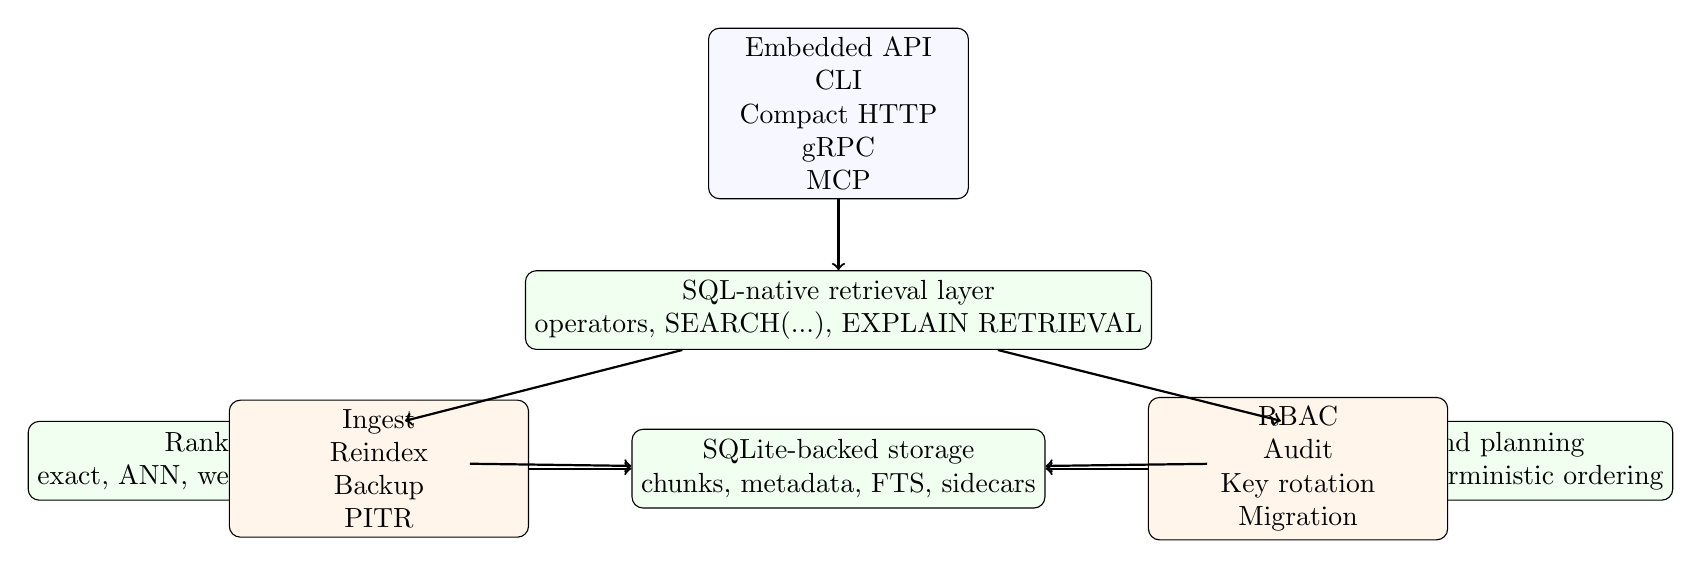
\begin{tikzpicture}[
      node distance=0.9cm and 0.7cm,
      box/.style={draw, rounded corners, align=center, minimum width=3.3cm, minimum height=0.9cm, fill=blue!3},
      core/.style={draw, rounded corners, align=center, minimum width=4.2cm, minimum height=1.0cm, fill=green!6},
      ops/.style={draw, rounded corners, align=center, minimum width=3.8cm, minimum height=0.9cm, fill=orange!8},
      line/.style={->, thick}
    ]
    \node[box] (surfaces) {Embedded API \\ CLI \\ Compact HTTP \\ gRPC \\ MCP};
    \node[core, below=of surfaces] (sql) {SQL-native retrieval layer \\ operators, SEARCH(...), EXPLAIN RETRIEVAL};
    \node[core, below left=of sql] (rank) {Ranking layer \\ exact, ANN, weighted fusion, RRF};
    \node[core, below right=of sql] (planner) {Execution and planning \\ query profiles, deterministic ordering};
    \node[core, below=1.0cm of sql] (storage) {SQLite-backed storage \\ chunks, metadata, FTS, sidecars};
    \node[ops, left=1.3cm of storage] (ops) {Ingest \\ Reindex \\ Backup \\ PITR};
    \node[ops, right=1.3cm of storage] (security) {RBAC \\ Audit \\ Key rotation \\ Migration};
    \draw[line] (surfaces) -- (sql);
    \draw[line] (sql) -- (rank);
    \draw[line] (sql) -- (planner);
    \draw[line] (rank) -- (storage);
    \draw[line] (planner) -- (storage);
    \draw[line] (ops) -- (storage);
    \draw[line] (security) -- (storage);
  \end{tikzpicture}
  }
  \caption{SQLRite architecture: a SQLite-backed retrieval core exposed through embedded and optional service surfaces.}
  \label{fig:architecture}
\end{figure}

\section{SQL-Native Retrieval Model}
SQLRite treats retrieval as part of the SQL surface rather than as a separate application API. The system exposes pgvector-style distance operators together with retrieval helper functions and a higher-level \texttt{SEARCH(...)} form.

\subsection{Distance Operators and Helper Functions}
SQLRite supports vector distance operators such as \texttt{<->}, \texttt{<=>}, and \texttt{<\#>} together with helper functions such as \texttt{vector(...)}, \texttt{embed(...)}, \texttt{bm25\_score(...)}, and \texttt{hybrid\_score(...)}. This makes it possible to express lexical, vector, and hybrid scoring directly in SQL.

\begin{lstlisting}[language=SQLRiteSQL, caption={Example hybrid retrieval query in SQLRite.}]
SELECT chunk_id, doc_id,
       hybrid_score(
         bm25_score(body, 'local memory'),
         1.0 / (1.0 + embedding <-> embed('local memory')),
         0.4,
         0.6
       ) AS score
FROM chunks
ORDER BY score DESC, chunk_id ASC
LIMIT 5;
\end{lstlisting}

\subsection{SEARCH and Explainability}
The higher-level \texttt{SEARCH(...)} form captures common retrieval intent, while \texttt{EXPLAIN RETRIEVAL} exposes planner choices. This matters for AI-agent systems because retrieval behavior influences downstream reasoning and tool selection. SQLRite therefore emphasizes deterministic tie-breaking and explicit planner visibility, not only raw ranking speed.

\section{Implementation}
SQLRite is implemented in Rust with SQLite as the storage substrate. The implementation integrates:
\begin{itemize}[leftmargin=*, itemsep=0.2em]
  \item exact vector search, ANN search, lexical search, and hybrid fusion,
  \item quantized vector storage options (\texttt{f32}, \texttt{f16}, \texttt{int8}),
  \item exact and ANN sidecar persistence,
  \item embedded APIs and CLI tooling,
  \item compact HTTP, full HTTP, gRPC, and MCP surfaces,
  \item migration, backup, restore, compaction, audit, RBAC, and key-rotation workflows.
\end{itemize}

This breadth is a deliberate design choice. A local-first retrieval system is attractive only if it remains practical to package, migrate, inspect, and operate.

\section{Evaluation Methodology}
This paper reports two evidence families.

\subsection{Embedded Competitive Snapshot}
The first evaluation is a deterministic filtered cosine benchmark that reflects SQLRite's current strongest deployment path. The workload consists of 5,000 records, 120 measured queries, 64-dimensional vectors, exact tenant filtering across 8 tenants, and \(k=10\) retrieval. We report SQLRite in two deployment modes: embedded and compact HTTP. We also report comparator throughput on the same workload for sqlite-vec, pgvector, Qdrant, and LanceDB, using the current repository benchmark snapshot captured in \texttt{papers/sqlrite\_arxiv/embedded\_competitive\_snapshot.json}.

The intention of this benchmark is not to claim universal superiority across all deployment models. The intention is to measure SQLRite in the regime it is designed for and to compare that result against nearby systems under the same workload definition.

\subsection{Public Dataset Benchmark}
The second evaluation uses BEIR/SciFact with deterministic hashed dense embeddings over the same text content for all systems. This benchmark is fully local and reproducible. Exact vector retrieval is compared across SQLRite, sqlite-vec, and pgvector. Hybrid lexical+vector retrieval is compared across SQLRite and pgvector using the refreshed paper-local harness stored in \texttt{papers/sqlrite\_arxiv/run\_public\_dataset\_eval.py}. The updated results are stored in \texttt{papers/sqlrite\_arxiv/public\_dataset\_results.json}.

This second benchmark contributes judged relevance and a public corpus. It also provides a check that SQLRite's hybrid retrieval semantics are meaningful outside synthetic nearest-neighbor workloads.

\section{Results}
\subsection{Embedded-First Performance Snapshot}
Table~\ref{tab:sqlritepaths} reports SQLRite's own deployment-path results on the deterministic filtered workload.

\begin{table}[H]
  \centering
  \small
  \caption{SQLRite deployment-path results on the deterministic filtered cosine workload (5k records, 120 queries, 64 dimensions, 8 tenants, \(k=10\)).}
  \label{tab:sqlritepaths}
  \begin{tabular}{lrrr}
    \toprule
    Mode & QPS & p95 latency (ms) & Recall@10 \\
    \midrule
    brute\_force embedded & 3380.07 & 0.3543 & 1.0 \\
    hnsw\_baseline embedded & 3530.96 & 0.3327 & 1.0 \\
    brute\_force compact HTTP & 1807.27 & 0.7538 & 1.0 \\
    hnsw\_baseline compact HTTP & 1828.17 & 0.7070 & 1.0 \\
    \bottomrule
  \end{tabular}
\end{table}

These results matter for two reasons. First, they confirm that SQLRite is strongest when embedded, which matches the product's intended use. Second, they show that compact HTTP preserves a substantial share of embedded performance, which is relevant for agent runtimes that still need a lightweight service boundary.

Table~\ref{tab:exactsnapshot} reports the exact filtered snapshot against nearby systems. Table~\ref{tab:approxsnapshot} reports the approximate filtered snapshot.

\begin{table}[H]
  \centering
  \small
  \caption{Exact filtered cosine throughput snapshot on the same workload.}
  \label{tab:exactsnapshot}
  \begin{tabular}{lr}
    \toprule
    System & QPS \\
    \midrule
    SQLRite brute\_force embedded & 3380.07 \\
    sqlite-vec exact & 3163.27 \\
    Qdrant exact & 2576.75 \\
    pgvector exact & 1739.64 \\
    LanceDB exact & 1063.08 \\
    \bottomrule
  \end{tabular}
\end{table}

\begin{table}[H]
  \centering
  \small
  \caption{Approximate filtered cosine snapshot on the same workload.}
  \label{tab:approxsnapshot}
  \begin{tabular}{lrr}
    \toprule
    System & QPS & Recall@10 \\
    \midrule
    SQLRite hnsw\_baseline embedded & 3530.96 & 1.0 \\
    Qdrant HNSW & 2661.91 & 1.0 \\
    pgvector HNSW & 1924.01 & 0.5740 \\
    LanceDB IVF\_FLAT & 1331.18 & 0.9510 \\
    \bottomrule
  \end{tabular}
\end{table}

The correct interpretation is specific. On this workload, SQLRite now leads the embedded filtered benchmark snapshot in both exact and approximate mode. That is a materially different result from earlier revisions of the system, where SQLRite trailed specialized engines on raw filtered-vector throughput. It would still be a mistake to generalize this into a universal claim. The current evidence shows benchmark leadership on this workload and in this deployment regime, not across all corpora, all dimensions, or all service configurations.

\subsection{Public Dataset Results}
Table~\ref{tab:publicexact} reports exact vector retrieval on BEIR/SciFact. Table~\ref{tab:publichybrid} reports hybrid lexical+vector retrieval on the same corpus.

\begin{table}[H]
  \centering
  \small
  \caption{Public exact-vector benchmark on BEIR/SciFact (5,183 documents, 100 queries, 128 dimensions, \(k=10\)).}
  \label{tab:publicexact}
  \begin{tabular}{lrrrrrr}
    \toprule
    System & QPS & p50 ms & p95 ms & Recall@10 & MRR@10 & NDCG@10 \\
    \midrule
    SQLRite brute\_force compact HTTP & 204.76 & 4.018 & 6.773 & 0.2278 & 0.1424 & 0.1594 \\
    sqlite-vec exact & 2297.83 & 0.395 & 0.519 & 0.2278 & 0.1424 & 0.1594 \\
    pgvector exact & 569.76 & 1.521 & 3.458 & 0.2278 & 0.1424 & 0.1594 \\
    \bottomrule
  \end{tabular}
\end{table}

\begin{table}[H]
  \centering
  \small
  \caption{Public hybrid lexical+vector benchmark on the same SciFact workload.}
  \label{tab:publichybrid}
  \begin{tabular}{lrrrrrr}
    \toprule
    System & QPS & p50 ms & p95 ms & Recall@10 & MRR@10 & NDCG@10 \\
    \midrule
    SQLRite hybrid compact HTTP & 55.60 & 16.296 & 19.511 & 0.4028 & 0.4056 & 0.3973 \\
    pgvector hybrid & 23.66 & 30.010 & 112.778 & 0.2278 & 0.1442 & 0.1609 \\
    \bottomrule
  \end{tabular}
\end{table}

The exact-vector SciFact result is straightforward: exact retrieval produces the same effectiveness metrics across all three systems because the benchmark uses the same deterministic dense representation and exact nearest-neighbor ranking. SQLRite trails sqlite-vec and pgvector in exact-vector throughput in this public harness.

The hybrid result is more interesting. SQLRite hybrid retrieval improves Recall@10 from 0.2278 to 0.4028 and NDCG@10 from 0.1594 to 0.3973 relative to its own exact-vector baseline, while also exceeding the pgvector hybrid baseline on both throughput and effectiveness in this harness. This suggests that SQLRite's integrated hybrid retrieval path is not only a usability feature; it can produce a materially better operating point on a judged public dataset.

\subsection{Where SQLRite Wins Beyond Throughput}
SQLRite is not only a benchmark result. Its broader differentiation is that it joins embedded execution, SQL-native retrieval, and operational completeness inside one product boundary.

\begin{table}[H]
  \centering
  \small
  \caption{Capability dimensions where SQLRite is differentiated beyond raw throughput.}
  \label{tab:capabilities}
  \begin{tabularx}{\textwidth}{p{4.1cm}cccc}
    \toprule
    Capability & SQLRite & sqlite-vec & pgvector & Qdrant \\
    \midrule
    Embedded local-first default & Yes & Yes & No & No \\
    SQL-native retrieval syntax beyond distance operators & Yes & Partial & Partial & No \\
    Single-product operational surface (migration, backup, restore, reindex, security) & Yes & No & Partial & Partial \\
    Multi-surface access (embedded, CLI, HTTP, compact HTTP, gRPC, MCP) & Yes & No & Partial & Partial \\
    Deterministic retrieval-focused developer workflow in one package & Yes & Partial & Partial & No \\
    \bottomrule
  \end{tabularx}
\end{table}

This capability view matters because system choice for AI-agent infrastructure is rarely made on QPS alone. Developer control, operational cost, deployment simplicity, and inspectability remain decisive factors.

\section{Discussion}
The updated evidence changes the paper's central argument in an important way. Earlier drafts could defend SQLRite mainly as an integrated local-first system with weaker raw vector throughput. The current evidence supports a stronger statement: SQLRite can now be both integrated and genuinely competitive on the embedded filtered workload it is designed for.

Three points are especially important.

First, \textbf{embedded-first really matters}. SQLRite's best numbers are not on the served path; they are in-process, which is consistent with the product's intended use. Second, \textbf{transport overhead is now manageable}. Compact HTTP cuts a significant amount of response overhead relative to richer JSON envelopes and preserves much more of the embedded engine's throughput. Third, \textbf{hybrid retrieval is an actual quality lever}. On SciFact, SQLRite hybrid retrieval moves to a meaningfully better quality-throughput region than the pgvector hybrid baseline in the same harness.

These are useful conclusions for system builders. They suggest that local-first retrieval no longer has to be framed as a concession made for convenience. In the case of SQLRite, embedded execution is both the operationally simplest path and the fastest current path.

\section{Limitations and Threats to Validity}
The current evaluation still has important limits.
\begin{itemize}[leftmargin=*, itemsep=0.2em]
  \item \textbf{Single-machine evidence.} The benchmark snapshot is measured on one local machine and should not be generalized to every hardware class.
  \item \textbf{Mixed comparator styles.} The exact and approximate snapshot compares an embedded-first engine with both embedded and service-oriented systems on the same workload. This is useful for practitioners, but it is not a pure apples-to-apples deployment comparison.
  \item \textbf{One public dataset.} BEIR/SciFact is a useful judged corpus, but it is only one retrieval task.
  \item \textbf{Deterministic local embeddings.} The public benchmark uses deterministic hashed embeddings for reproducibility, not a production neural embedding service.
  \item \textbf{Workload-specific leadership.} The current embedded benchmark leadership should be interpreted as a workload-specific result, not a blanket claim over all vector and hybrid retrieval systems.
\end{itemize}

These limitations should be stated plainly. They do not weaken the contribution of the paper; they define its scope correctly.

\section{Reproducibility and Availability}
The software is available at:
\begin{quote}
  \url{https://github.com/zavora-ai/SQLRite}
\end{quote}

The current paper revision is grounded in these repository-local artifacts:
\begin{itemize}[leftmargin=*, itemsep=0.2em]
  \item \texttt{papers/sqlrite\_arxiv/embedded\_competitive\_snapshot.json}
  \item \texttt{papers/sqlrite\_arxiv/embedded\_competitive\_snapshot.md}
  \item \texttt{papers/sqlrite\_arxiv/public\_dataset\_results.json}
  \item \texttt{papers/sqlrite\_arxiv/public\_dataset\_results.md}
  \item \texttt{papers/sqlrite\_arxiv/run\_public\_dataset\_eval.py}
\end{itemize}

The paper-specific build entry point is \texttt{papers/sqlrite\_arxiv/build.sh}.

\section{Conclusion}
SQLRite demonstrates that local-first retrieval for AI agents can be built as a coherent SQL-native system on top of SQLite without giving up serious performance in the embedded regime. The current evidence supports three claims. First, SQLRite's strongest deployment path is embedded execution, where it now leads the current deterministic filtered benchmark snapshot in both exact and approximate mode. Second, compact HTTP preserves a large share of that performance when a process boundary is required. Third, SQLRite's hybrid retrieval semantics can buy real quality gains on a judged public dataset, not only on synthetic workloads.

The broader contribution is therefore twofold: SQLRite is both a systems design for embedded-first retrieval and a practical product surface that joins retrieval, SQL, agent-facing interfaces, and operations into a single package. Future work should extend the public evaluation to more datasets and hardware classes, add tighter apples-to-apples service comparisons, and continue improving the served-path gap relative to the embedded engine.

\bibliographystyle{plainnat}
\bibliography{references}

\end{document}
